
%%%%%%%%%%%%%%%%%%%%%%%%%%%%%%%%%%%%%%%%%%%%%%%%%%%%%%%%%%%%%%%%%%%%%%%%%%%%%
%%%%% Basic C++ %%%%%%%%%%%%%%%%%%%%%%%%%%%%%%%%%%%%%%%%%%%%%%%%%%%%%%%%%%%%%
%%%%%%%%%%%%%%%%%%%%%%%%%%%%%%%%%%%%%%%%%%%%%%%%%%%%%%%%%%%%%%%%%%%%%%%%%%%%%
\begin{frame}
\pointedsl{
	Basics
}
\end{frame}

% TODO
% Content:
% 1. Variables (declaration, assignment, operations)
% 2. Types (list: char, short, int, float, double, bool, void; typedef)
% 3. Expressions (unary, binary, arithmetic, comparator, bitwise)
% 4. Conditions (if, else if, else)
% 5. Loops (for, while, do while)
% 6. Functions (declaration, definition, signature /!\ types -> diff fun)
% 7. Arrays

%%%%%%%%%%%%%%%%%%%%%%%%%%%%%%%%%%%%%%%%%%%%%%%%%%%%%%%%%%%%%%%%%%%%%%%%%%%%%
\lstset{language=C++,numbers=none}
\begin{frame}[fragile]
\frametitle{Declaration and definition}
\begin{lstlisting}
void process(int x); // declare a function
int x; // declare a variable
x = 10; // assign a value
process(x);
// declaration and definition
int sum(int a, int b){ return a + b; }
// declaration and assignment
int y = sum(x, 2);
\end{lstlisting}
\misc{
	Every variable, type or function must be declared before being used. They can then be defined anywhere.
	
	\textbf{Note}: variables automatically receive a default value corresponding to $0$.
}
\end{frame}

%%%%%%%%%%%%%%%%%%%%%%%%%%%%%%%%%%%%%%%%%%%%%%%%%%%%%%%%%%%%%%%%%%%%%%%%%%%%%
\begin{frame}[fragile]
\frametitle{Flow control}
\begin{center}
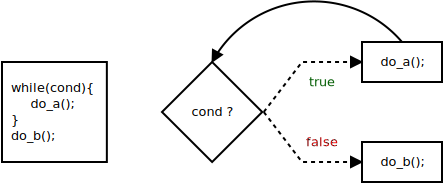
\includegraphics[width=0.7\textwidth]{figures/flow}
\end{center}
\misc{
	The usual conditional blocks are available
	\begin{itemize}
		\item \ctext{if}, \ctext{else if}, \ctext{else} and \ctext{switch}
	\end{itemize}
	as well as loop structures
	\begin{itemize}
		\item \ctext{for}, \ctext{while} and \ctext{do while}
	\end{itemize}
}
\end{frame}

%%%%%%%%%%%%%%%%%%%%%%%%%%%%%%%%%%%%%%%%%%%%%%%%%%%%%%%%%%%%%%%%%%%%%%%%%%%%%
\begin{frame}[fragile]
\frametitle{Arrays}
\begin{columns}[c]
  \begin{column}{0.5\textwidth}
\lstset{language=C++,numbers=left}
\begin{lstlisting}
int a[3] = { 1, 0 };
a[1] = 42;
// a[2] == 0
\end{lstlisting}
  \end{column}
  \begin{column}{0.5\textwidth}
    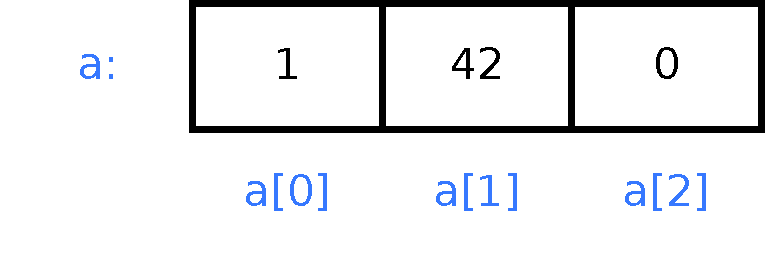
\includegraphics[width=0.95\textwidth]{figures/array0}
  \end{column}
\end{columns}
\misc{
	\emph{Arrays} are continuous blocks of memory that store multiple elements of a same type. They use $0$-based indexing.
}
\end{frame}
